\documentclass{article}

\usepackage{graphicx}
\usepackage{tikz}
\usepackage{tikzsymbols}
\usetikzlibrary{calc,patterns,shapes.geometric}
\pagestyle{empty}
\usepackage[margin=0pt]{geometry}
\geometry{papersize={14in,12in}}

\def\centerarc[#1](#2)(#3:#4:#5){\draw[#1] ($(#2)+({#5*cos(#3)},{#5*sin(#3)})$) arc (#3:#4:#5);}

\begin{document}
	\begin{figure}
		\centering
		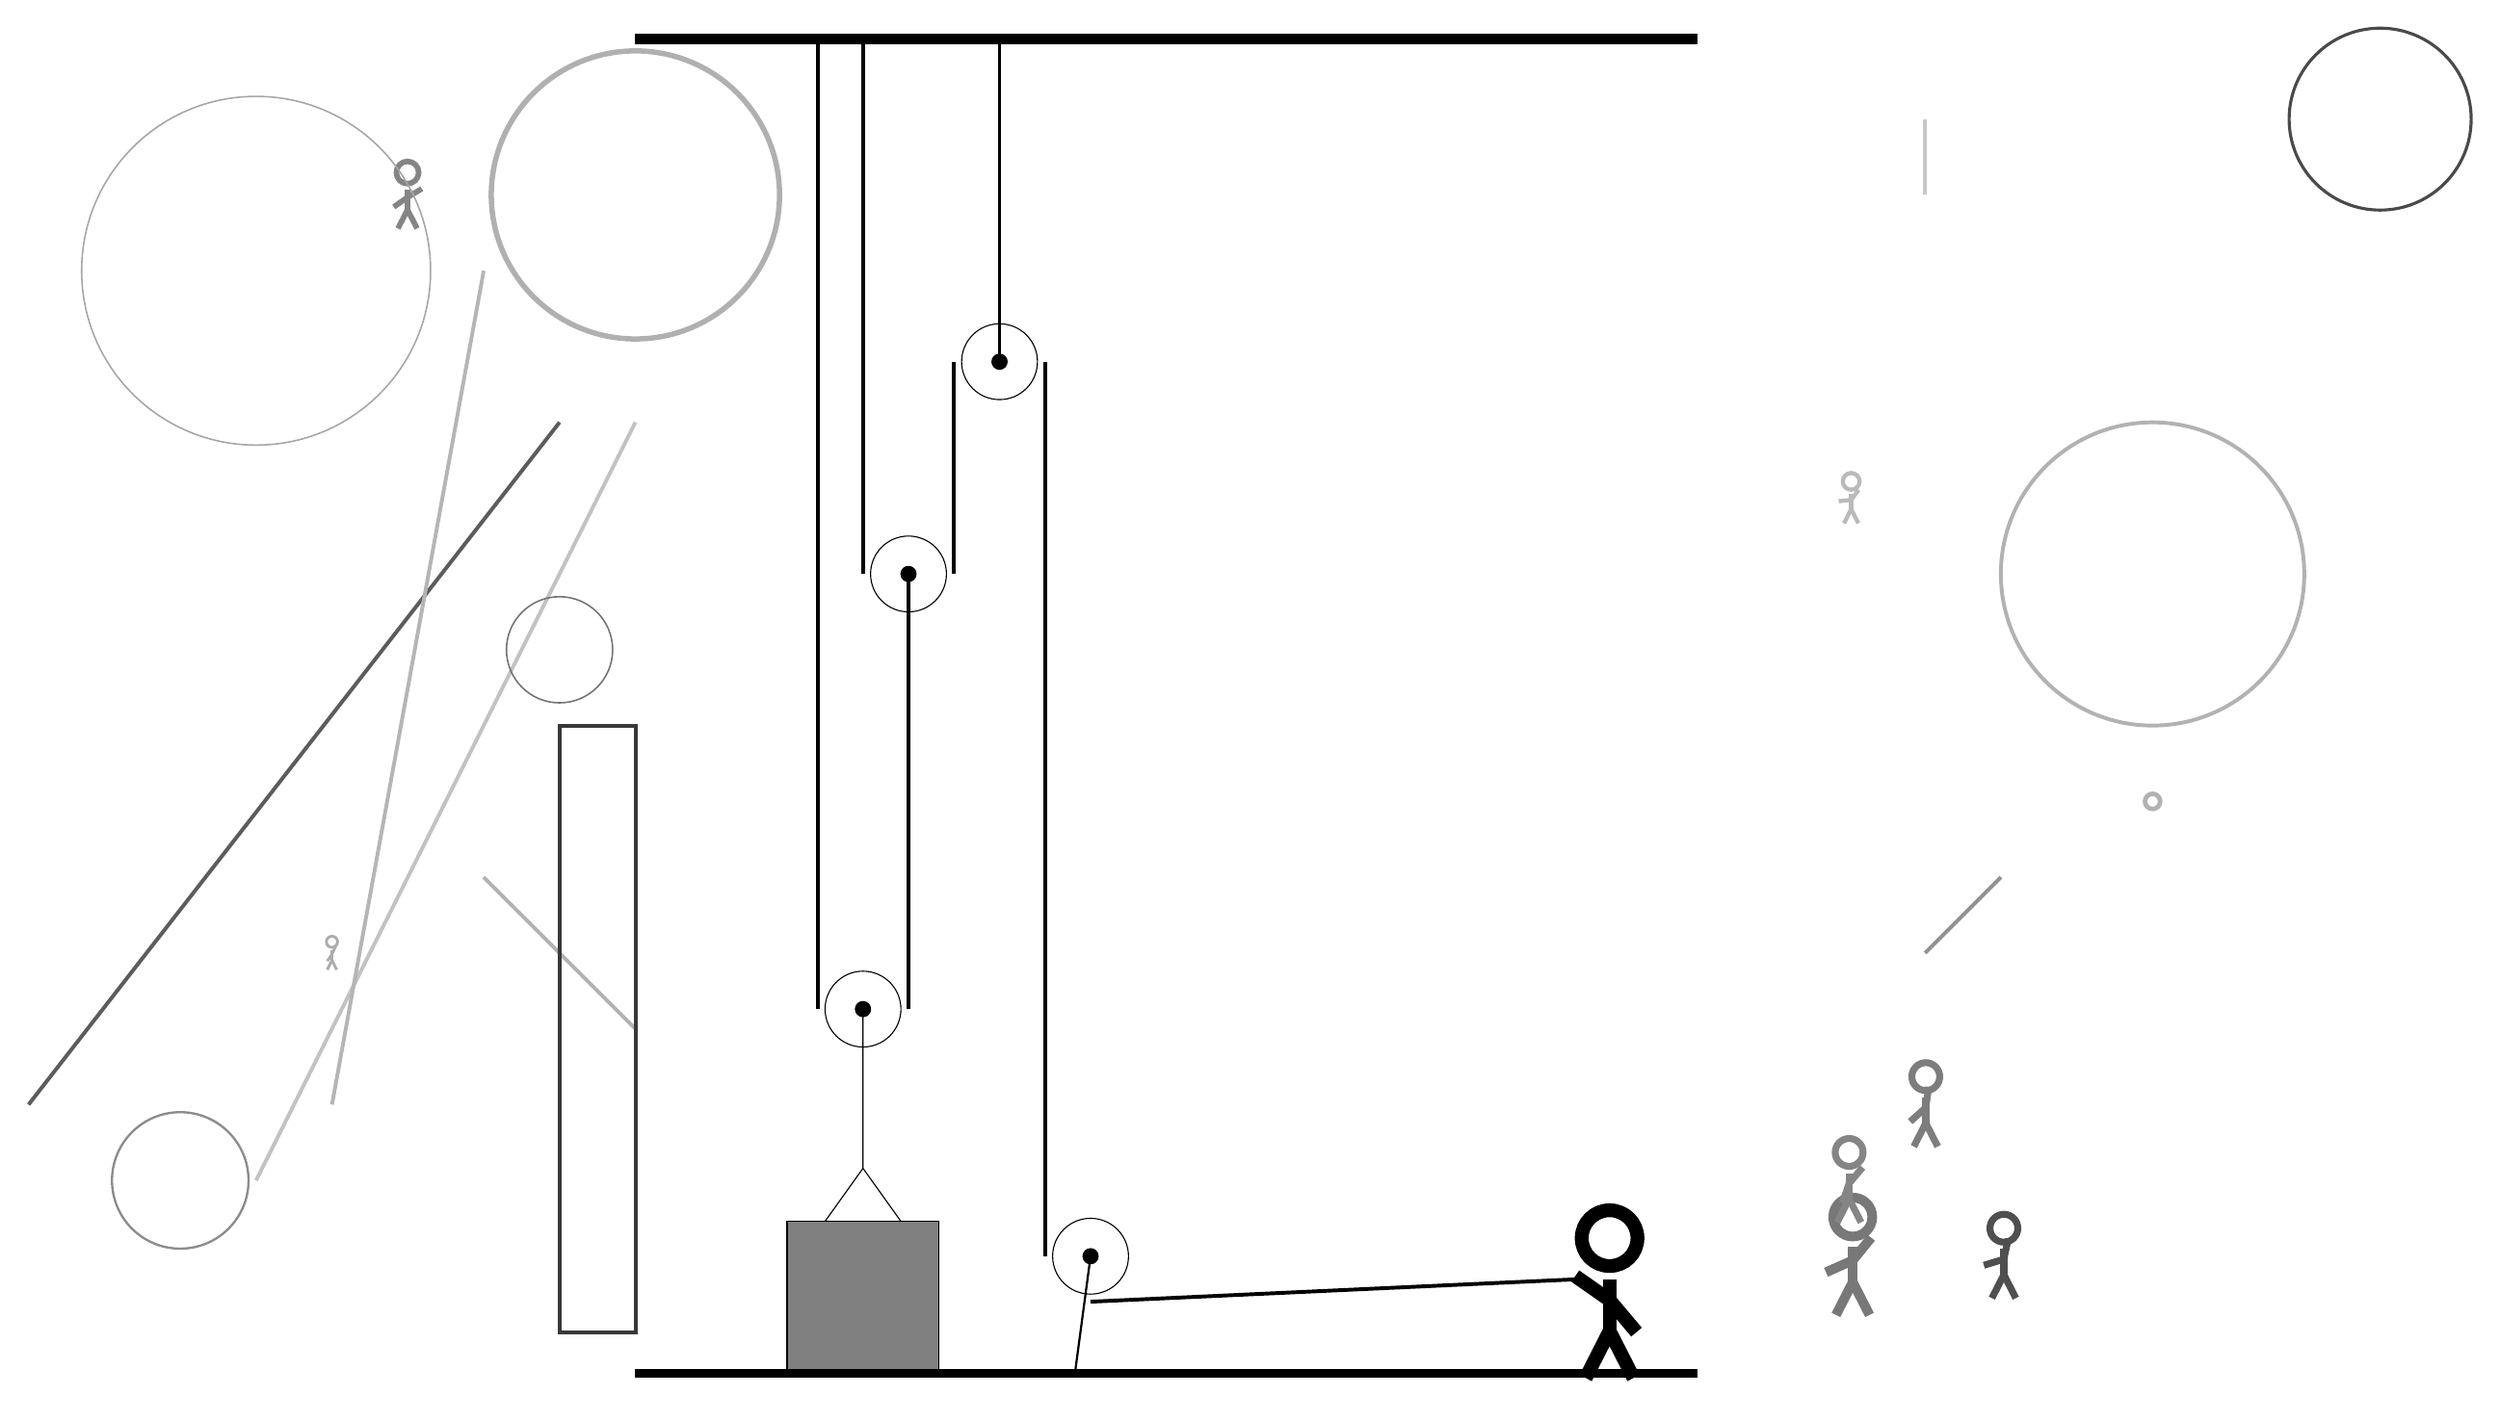
\begin{tikzpicture}
			%%%%% START %%%%%
			
			\draw[fill=black] (-2, 14) rectangle (12, 14.125);
			
			\node[line width=0.4mm, color=black!69] at (16, -2) {\Strichmaxerl[5][17][78]};
			
			\node[line width=0.4mm, color=black!48] at (-5, 12) {\Strichmaxerl[4][35][31]};
			\draw [line width=0.3mm, color=black!45](-8, -1) circle (0.9);
			\node[line width=0.4mm, color=black!27] at (14, 8) {\Strichmaxerl[3][6][54]};
			
			\draw[line width=0.5mm, color=black!24](-7, -1) -- (-2, 9);
			\node[line width=0.2mm, color=black!51] at (15, 0) {\Strichmaxerl[5][42][82]};
			
			\draw[line width=0.5mm, color=black!64](-3, 9) -- (-10, 0);
			
			\node[line width=0.2mm, color=black!33] at (-6, 2) {\Strichmaxerl[2][56][65]};
			\draw [line width=0.6mm, color=black!30](18, 4) circle (0.1);
			\draw[line width=0.5mm, color=black!30](-2, 1) -- (-4, 3);
			
			\draw[line width=0.5mm, color=black!22](15, 13) -- (15, 12);
			\node[line width=0.2mm, color=black!53] at (14, -2) {\Strichmaxerl[7][24][51]};
			\draw [line width=0.4mm, color=black!71](21, 13) circle (1.2);
			\draw[line width=0.5mm, color=black!29](-6, 0) -- (-4, 11);
			\draw[line width=0.5mm, color=black!43](16, 3) -- (15, 2);
			\node[line width=0.3mm, color=black!48] at (14, -1) {\Strichmaxerl[5][71][50]};
			\draw [line width=0.2mm, color=black!55](-3, 6) circle (0.7);
			
			\draw [line width=0.2mm, color=black!35](-7, 11) circle (2.3);
			\draw[line width=0.5mm, color=black!78] (-3, -3) rectangle (-2, 5);
			
			\draw [line width=0.7mm, color=black!31](-2, 12) circle (1.9);
			\draw [line width=0.5mm, color=black!30](18, 7) circle (2.0);
			
			
			\draw (1, 1.26) circle (0.5);
			\draw[fill=black] (1, 1.26) circle (0.1);
			
			\draw (1.6, 7.0) circle (0.5);
			\draw[fill=black] (1.6, 7.0) circle (0.1);
			
			\draw (2.8, 9.8) circle (0.5);
			\draw[fill=black] (2.8, 9.8) circle (0.1);
			\draw[thick] (2.8, 9.8) -- (2.8, 14);
			
			\draw (4.0, -2) circle (0.5);
			\draw[fill=black] (4.0, -2) circle (0.1);
			\draw[thick] (4.0, -2) -- (3.8, -3.5);
			
			\draw (1, 1.26) -- (1, -0.84) -- (0.5, -1.54) -- (1.5, -1.54) -- (1, -0.84);
			\draw[fill=black!50] (0, -1.54) rectangle (2, -3.54);
			\draw[line width=0.5mm] (0.4, 14) -- (0.4, 1.26);
			\centerarc[line width=0.5mm](1, 1.26)(180:360:0.6);
			\draw[line width=0.5mm](1.6, 1.26) -- (1.6, 7.0);
			\draw[line width=0.5mm] (1.0, 14) -- (1.0, 7.0);
			\centerarc[line width=0.5mm](1.6, 7.0)(180:360:0.6);
			\draw[line width=0.5mm](2.2, 7.0) -- (2.2, 9.8);
			\centerarc[line width=0.5mm](2.8, 9.8)(0:180:0.6);
			\draw[line width=0.5mm] (3.4, 9.8) -- (3.4, -2);
			\centerarc[line width=0.5mm](4.0, -2)(0:90:-0.6);
			\draw[line width=0.5mm](4.0, -2.6) -- (10.5, -2.3);
			
			\node at (10.8, -2.5) {\Strichmaxerl[10][-35][-50]};
			
			\draw[fill=black] (-2, -3.5) rectangle (12, -3.6);
			
			%%%%% END %%%%%
		\end{tikzpicture}
	\end{figure}	
\end{document}